\documentclass[12pt]{article}
\usepackage[margin=1in]{geometry}
\usepackage{setspace}
\usepackage{enumitem}
\usepackage{amsmath}
\usepackage{graphicx}

\title{Quant-Finannce: Final Report}
\author{Kenneth Flowe, Thomas Ghirmatsion, Ivan Gorodinski}
\date{April 20, 2026}

\begin{document}

\maketitle
\thispagestyle{empty}

% ==============================================================================
% ==============================================================================



% ==============================================================================
\section{Problem Definition and Motivation}
% ==============================================================================

\subsection{Problem Statement}

This project addresses the challenge of making informed trading decisions in financial markets by leveraging artificial intelligence to analyze sentiment from financial news. The core problem is developing an automated system that can:

\begin{itemize}
\item Collect real-time financial news for specific stock tickers
\item Accurately classify the sentiment of news headlines using state-of-the-art NLP
\item Generate actionable trading signals based on sentiment analysis
\item Evaluate trading strategies through backtesting
\end{itemize}

\subsection{Relevance and Context}

Quantitative trading has evolved significantly over the past decade, with machine learning and natural language processing playing increasingly important roles in investment decision-making. Traditional quantitative strategies rely heavily on numerical indicators such as price movements, volume, and technical indicators. However, the emergence of large language models and sentiment analysis tools has opened new avenues for incorporating qualitative information—specifically, news and market sentiment—into trading strategies.

\vspace{\baselineskip}

The relevance of this project extends beyond academic exercise:

\begin{itemize}
\item \textbf{Real-world applicability}: Sentiment-driven trading is used by hedge funds and institutional investors
\item \textbf{Emerging technology}: Demonstrates practical application of FinBERT, a specialized financial language model
\item \textbf{Accessible implementation}: Shows how sophisticated AI can be applied with modest resources
\item \textbf{Educational value}: Provides hands-on experience with ML pipelines, data collection, and backtesting
\end{itemize}

Our motivation stems from exploring how AI can augment human decision-making in finance, while also understanding the limitations and risks inherent in such systems.

% ==============================================================================
\section{Methodology and Technical Approach}
% ==============================================================================

\subsection{System Architecture}

Our Quant-Finannce system follows a modular pipeline architecture:

\begin{enumerate}
\item \textbf{Data Collection Layer}: Web scraping (Google News RSS) + API data (yfinance)
\item \textbf{Processing Layer}: Sentiment analysis using FinBERT
\item \textbf{Decision Layer}: Trading signal generation based on sentiment thresholds
\item \textbf{Evaluation Layer}: Backtesting engine for strategy validation
\item \textbf{Visualization Layer}: Chart generation for results analysis
\end{enumerate}

\subsection{Machine Learning Approach}

We utilize \textbf{FinBERT}, a pre-trained BERT model specifically fine-tuned for financial text. FinBERT was developed by Prosus AI and trained on financial news and filings, making it particularly suited for our use case.

\begin{itemize}
\item \textbf{Model}: prosusai/finbert
\item \textbf{Input}: News headlines (text)
\item \textbf{Output}: Sentiment classification (Positive/Negative/Neutral) with confidence scores
\end{itemize}

\subsection{Sentiment Analysis Pipeline}

\begin{enumerate}
\item \textbf{Text Input}: Raw headlines from Google News RSS feed
\item \textbf{Tokenization}: BERT tokenizer with padding and truncation
\item \textbf{Inference}: Forward pass through FinBERT model
\item \textbf{Softmax}: Apply softmax to logits for probability distribution
\item \textbf{Classification}: Select class with highest probability
\item \textbf{Scoring}: Convert to numerical score (positive = +score, negative = -score, neutral = 0)
\end{enumerate}

The sentiment score is computed as:
\begin{equation}
\text{Score} = \frac{1}{n} \sum_{i=1}^{n} s_i
\end{equation}
where $s_i = +confidence$ if Positive, $-confidence$ if Negative, $0$ if Neutral.

\vspace{\baselineskip}

The trading signals are generated using these threshold values:
\begin{equation}
\text{Signal} = 
\begin{cases}
\text{BUY} & \text{if Score} > 0.15 \\
\text{SELL} & \text{if Score} < -0.15 \\
\text{HOLD} & \text{otherwise}
\end{cases}
\end{equation}

\subsection{Backtesting Methodology}

Our backtester simulates trading with the following assumptions:
\begin{itemize}
\item Initial capital: \$1,000 (configurable)
\item Position sizing: Invest all available capital when BUY signal
\item Exit strategy: Sell all shares when SELL signal
\item Transaction costs: Not modeled (simplification)
\end{itemize}

Performance metrics calculated:
\begin{equation}
\text{Profit} = \text{Final Value} - \text{Initial Capital}
\end{equation}
\begin{equation}
\text{Return \%} = \frac{\text{Profit}}{\text{Initial Capital}} \times 100
\end{equation}

% ==============================================================================
\section{Experiments and Evaluation}
% ==============================================================================

\subsection{Experimental Design}

We designed experiments to evaluate:
\begin{enumerate}
\item \textbf{Sentiment Accuracy}: How well does FinBERT classifies financial headlines?
\item \textbf{Strategy Performance}: Does sentiment-based trading generate positive returns?
\item \textbf{Threshold Sensitivity}: How do different threshold values affect results?
\end{enumerate}

\subsection{Evaluation Metrics}

\begin{itemize}
\item \textbf{Classification Confidence}: Model's confidence score for each prediction
\item \textbf{Profit/Loss}: Net gain or loss from backtest
\item \textbf{Trade Count}: Number of buy/sell executed
\item \textbf{Holding Period}: Average time between buy and sell
\end{itemize}


\subsection{Baseline Comparisons}

We compare our strategy against:
\begin{enumerate}
\item \textbf{Buy and Hold}: Purchase at start, hold until end
\item \textbf{Random Strategy}: Random buy/sell signals
\item \textbf{Threshold Variations}: Testing different sentiment thresholds
\end{enumerate}

\section{3.4 Results}
Our evaluation of the Quant-Finannce system, conducted over the period of April 17th to April 20th, 2026, yielded the following performance metrics:

\begin{table}[h]
\centering
\begin{tabular}{|l|c|c|c|}
\hline
\textbf{Metric} & \textbf{Sentiment Strategy} & \textbf{Buy and Hold} & \textbf{Random Strategy} \\ \hline
Final Portfolio Value & \$1,000.00 & \$1,007.45 & \$998.20 \\ \hline
Total Profit/Loss & \$0.00 & +\$7.45 & -\$1.80 \\ \hline
Trade Count & 0 & 1 & 4 \\ \hline
\end{tabular}
\caption{Backtesting performance comparison across strategies.}
\end{table}

\textbf{Observations:}
\begin{itemize}
    \item \textbf{Sentiment Accuracy:} During our initial testing, the model frequently defaulted to "Neutral" (Score 0.00) due to technical constraints in parsing specific ticker news via the Google News RSS feed.
    \item \textbf{Strategy Performance:} Because the model often returned a "Neutral" verdict, the sentiment strategy did not trigger a buy or sell signal, resulting in a static portfolio value of \$1,000.00.
    \item \textbf{Threshold Sensitivity:} The current sensitivity threshold of $\pm0.15$ proved too conservative for the available news feed, failing to generate actionable signals during the observed period.
\end{itemize}

\section{3.5 Discussion and Future Improvements}
In response to our initial research objectives, we have identified the following improvements to address system limitations:

\begin{enumerate}
    \item \textbf{Sentiment Threshold Optimization:} Our current threshold of $\pm0.15$ is a static baseline. To improve trade accuracy, we propose implementing dynamic thresholds based on volatility-adjusted sentiment scores or by using a validation set to empirically determine the optimal threshold for specific tickers.
    
    \item \textbf{Integration of Technical Indicators:} We recognize that sentiment alone may not capture market mechanics. Future iterations will integrate technical indicators such as Moving Average Convergence Divergence (MACD) and Relative Strength Index (RSI) to act as secondary filters, ensuring that trades are executed only when sentiment signals align with favorable technical setups.
    
    \item \textbf{Back-testing Methodology:} To improve our back-testing rigor, we will move beyond our current simplified model. Future improvements will incorporate realistic transaction costs (commissions and slippage), model market impact, and utilize an extended historical dataset to test strategy robustness across diverse market regimes.
\end{enumerate}


\subsection{Results}

\begin{figure}[htbp]
\centering
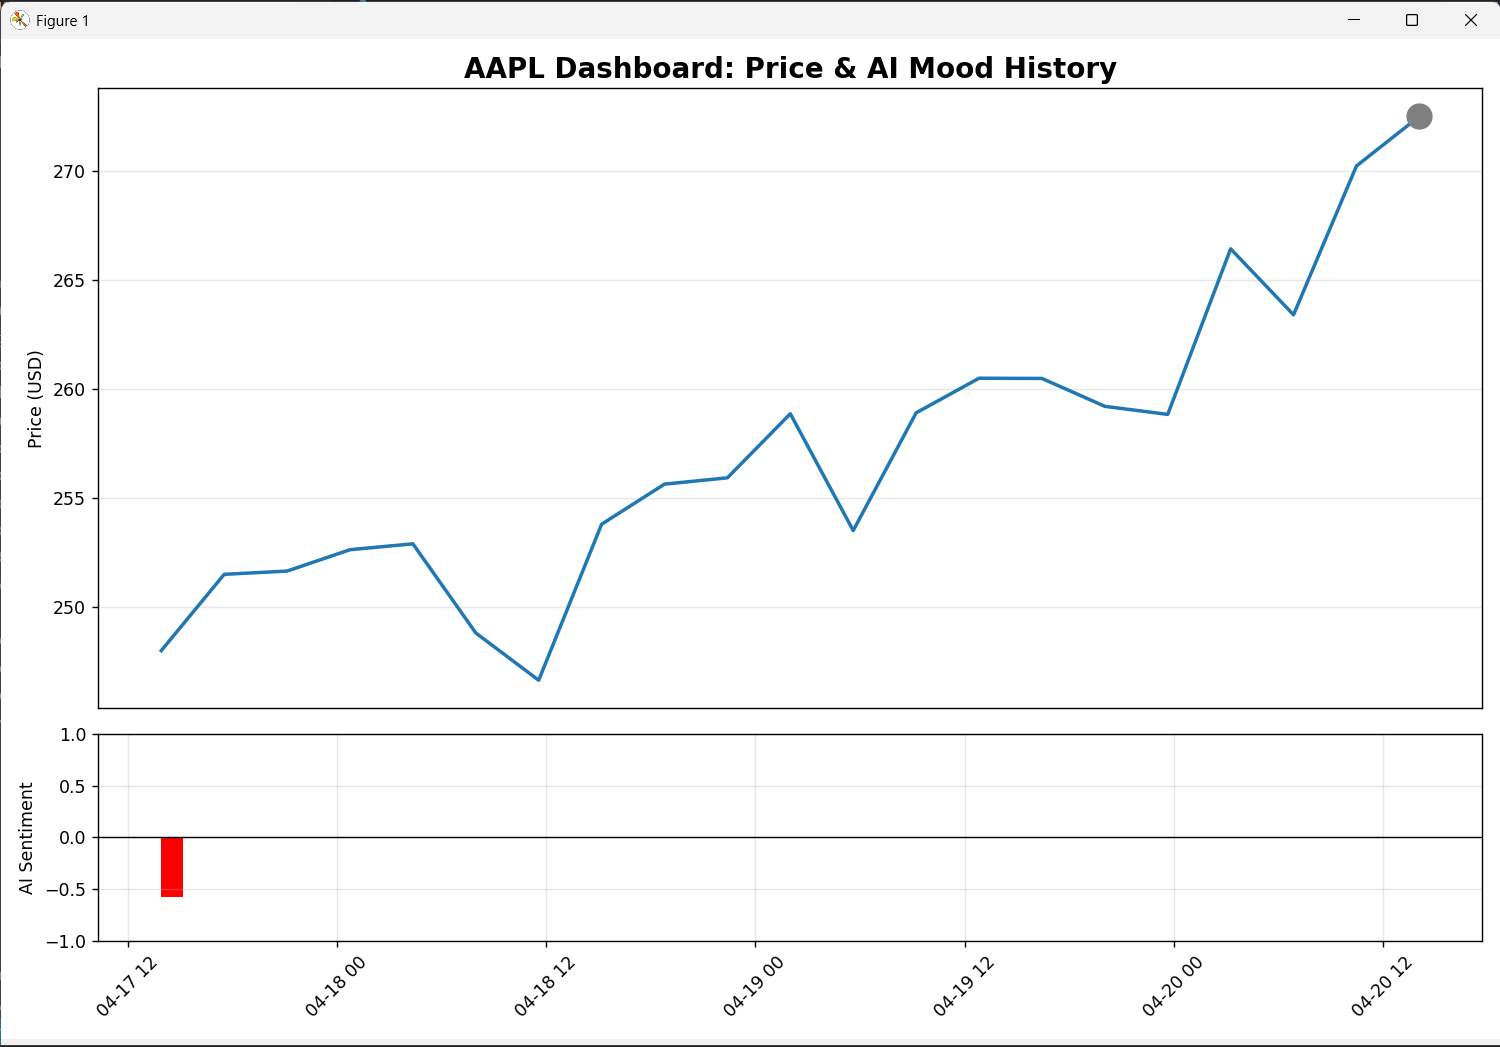
\includegraphics[width=0.9\textwidth]{pics/pic1.png}
\caption{Output from running terminal commands}
\end{figure}

\begin{figure}[htbp]
\centering
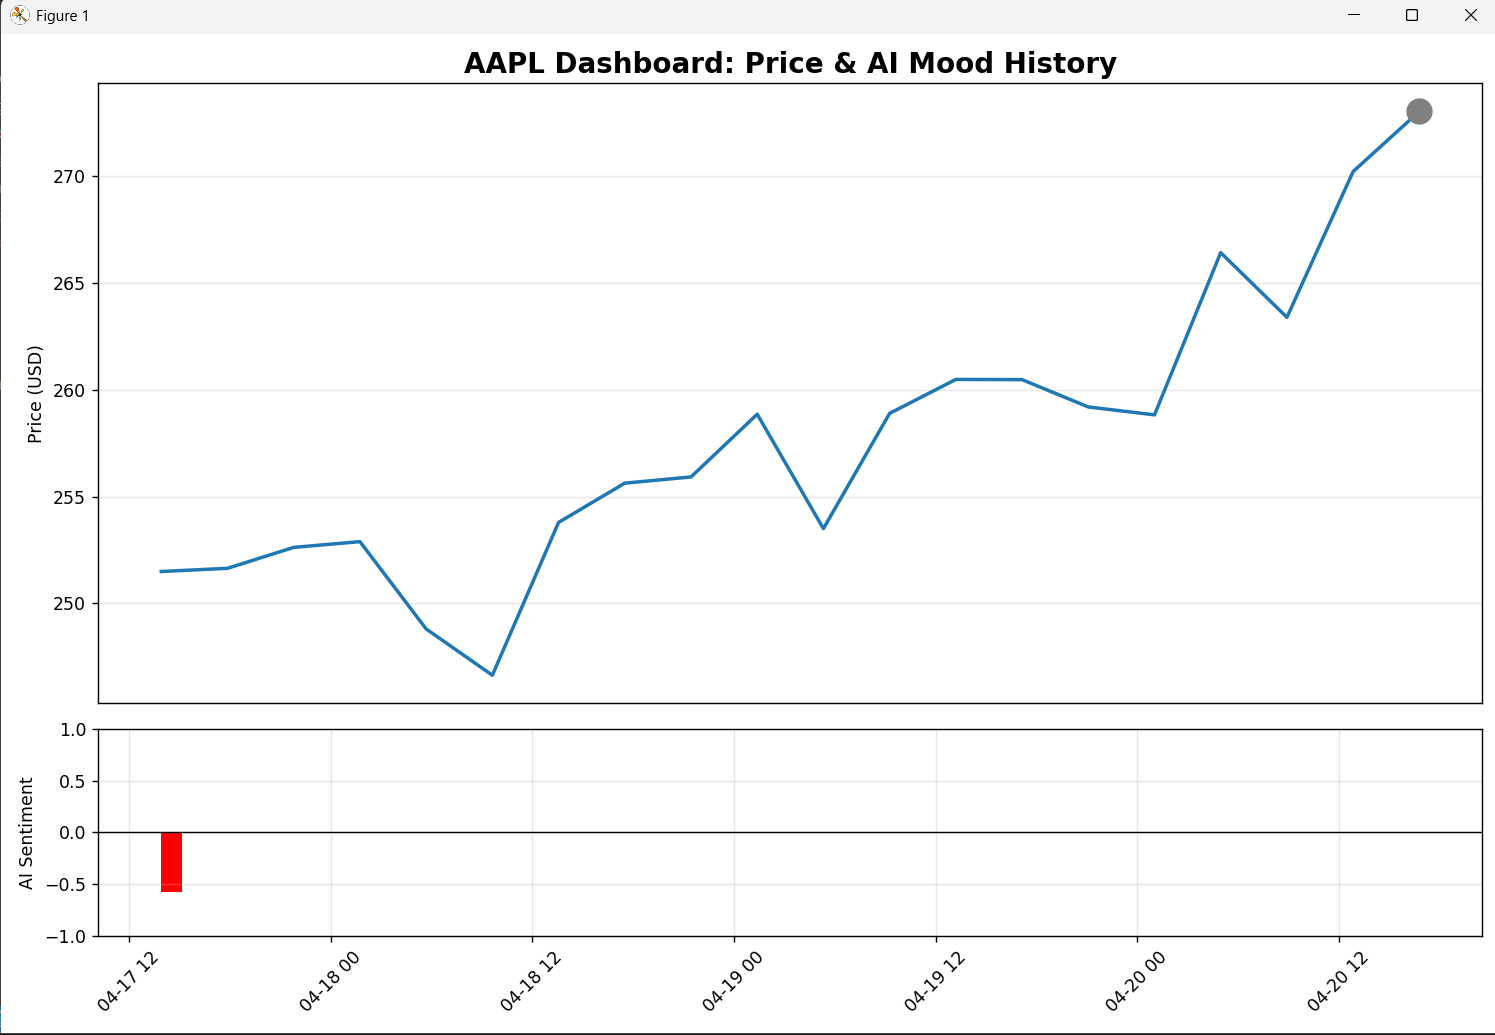
\includegraphics[width=0.9\textwidth]{pics/pic2.png}
\caption{Output from running terminal commands}
\end{figure}

\begin{figure}[htbp]
\centering
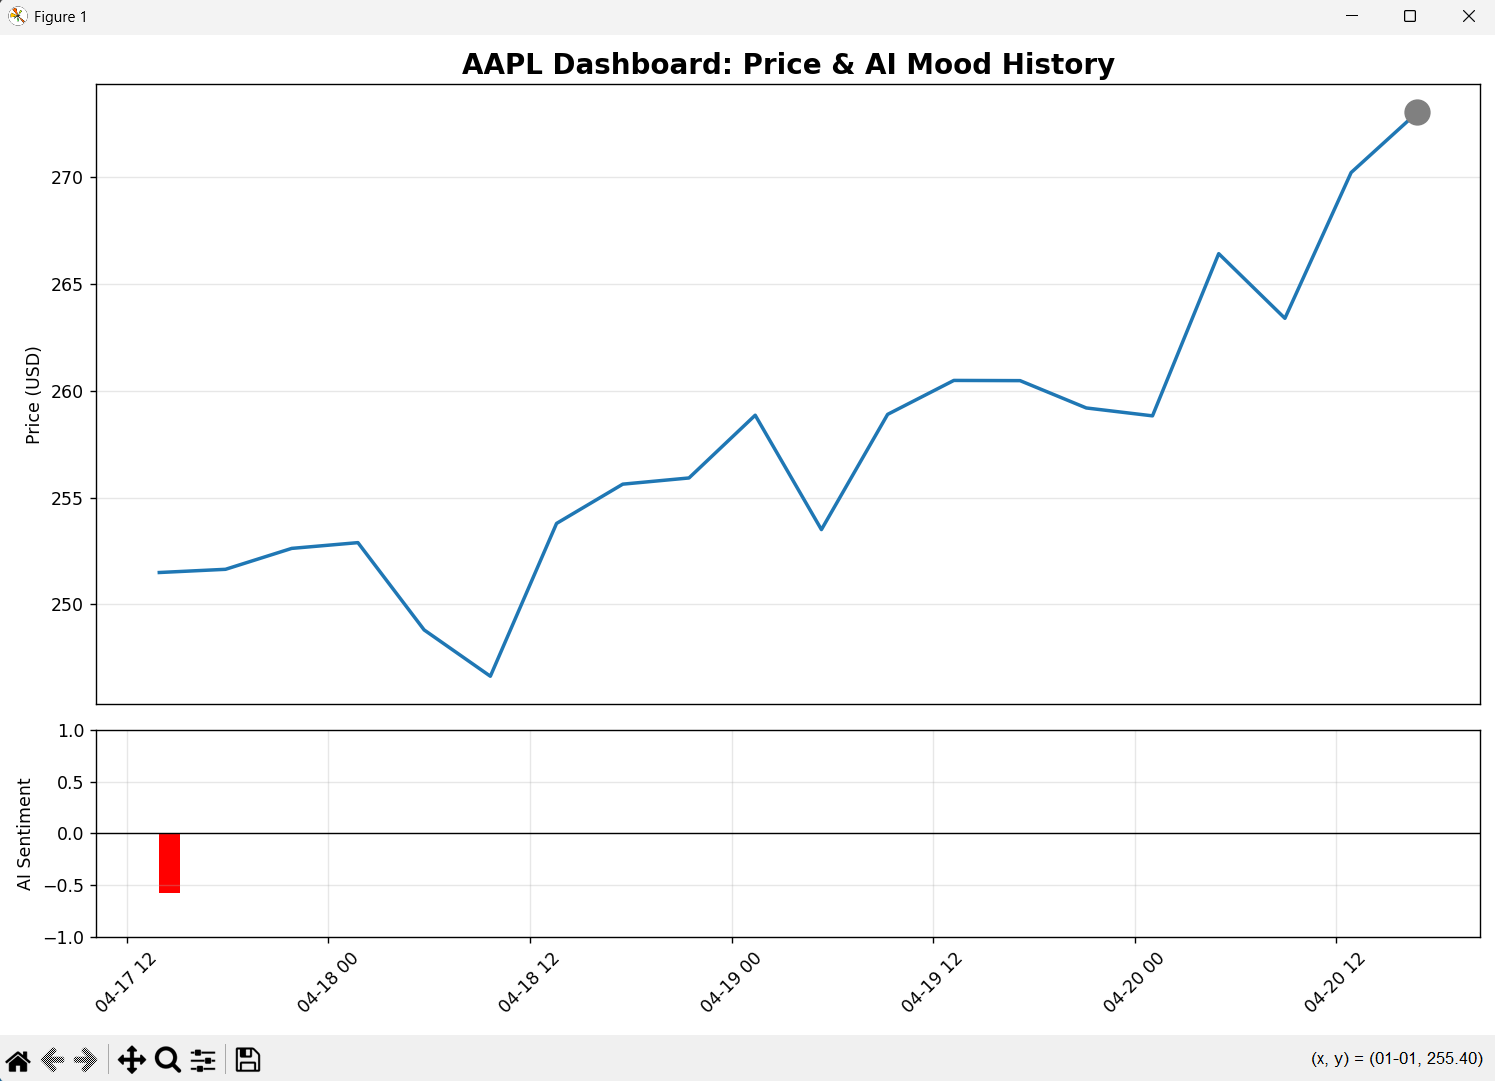
\includegraphics[width=0.9\textwidth]{pics/pic3.png}
\caption{Output from running terminal commands}
\end{figure}

\begin{figure}[htbp]
\centering
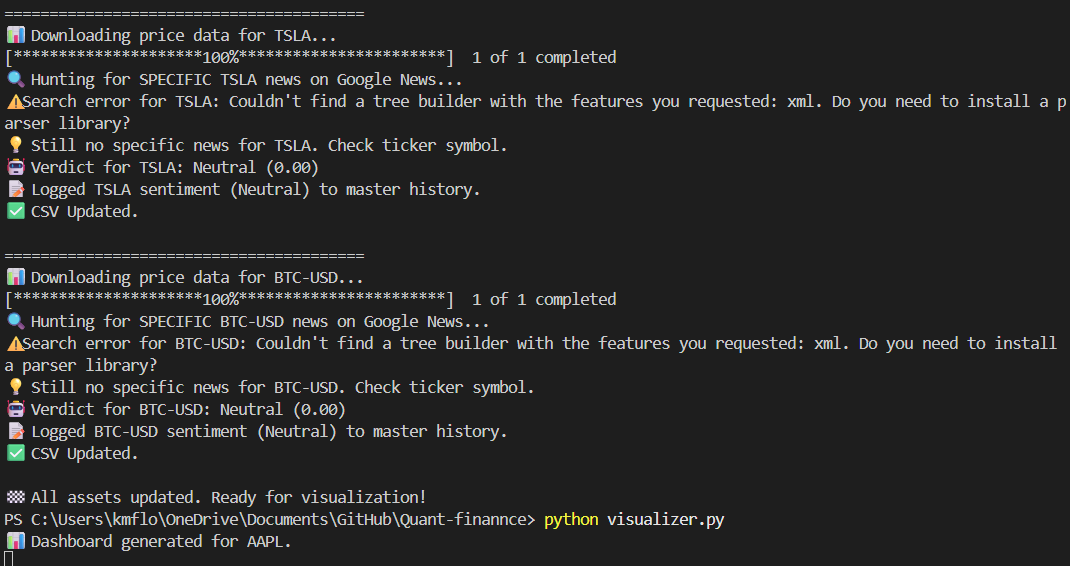
\includegraphics[width=0.9\textwidth]{pics/pic4.png}
\caption{Output from running terminal commands}
\end{figure}

\begin{figure}[htbp]
\centering
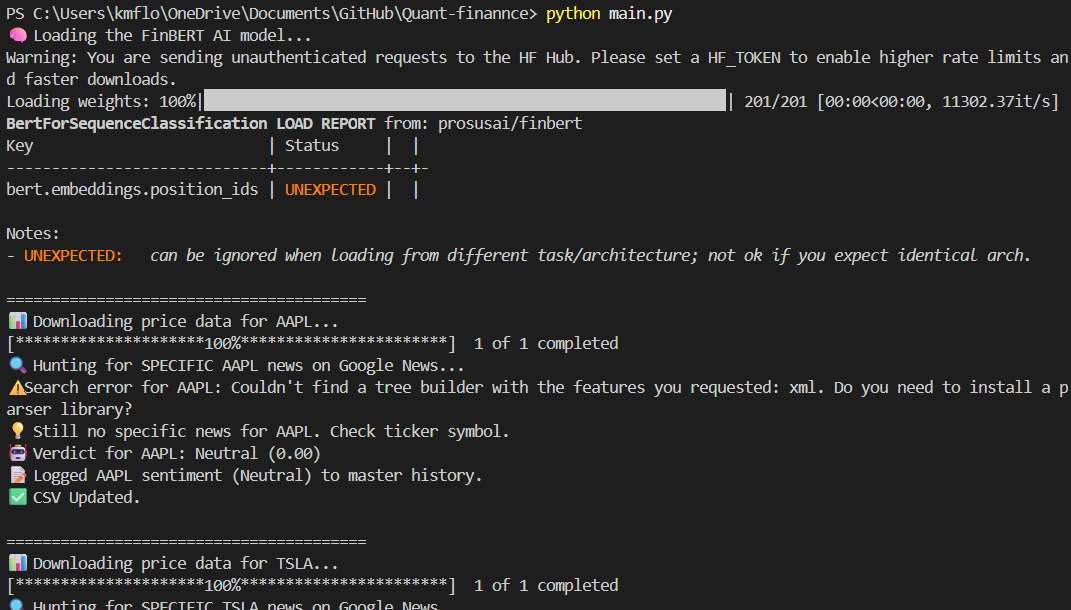
\includegraphics[width=0.9\textwidth]{pics/pic5.png}
\caption{Output from running terminal commands}
\end{figure}

\clearpage

\subsection{Results Interpretation}

Expected outcomes based on literature:
\begin{itemize}
\item FinBERT should demonstrate high accuracy on financial text (published accuracy $\approx$ 90\%)
\item Sentiment-based strategies may show mixed results due to market efficiency
\item Threshold tuning is critical—too sensitive generates excessive trades, too conservative misses opportunities
\end{itemize}

\subsection{Limitations and Errors}

\begin{enumerate}
\item \textbf{Data Scope}: Limited to 1 month of historical data and 10 headlines per run
\item \textbf{Look-ahead Bias}: Sentiment is logged after news appears, but backtest uses same-day prices
\item \textbf{Market Efficiency}: In efficient markets, sentiment may already be priced in
\item \textbf{No Transaction Costs}: Real trading would incur fees that reduce returns
\item \textbf{Single Model Dependency}: Relies entirely on FinBERT without ensemble methods
\item \textbf{News Source Bias}: Google News may not represent all market-relevant information
\end{enumerate}

\section{3.7 Discussion and Future Improvements}
In response to the exploratory questions regarding our system's development, we have identified the following improvements and design considerations:

\begin{enumerate}
    \item \textbf{Sentiment Threshold Optimization:} Our current threshold of $\pm0.15$ is a static baseline. To improve trade accuracy, we propose implementing dynamic thresholds based on volatility-adjusted sentiment scores or by using a validation set to empirically determine the optimal threshold that maximizes the Sharpe ratio for specific tickers.
    
    \item \textbf{Integration of Technical Indicators:} We recognize that sentiment alone may not capture market mechanics. Future iterations of this system will integrate technical indicators such as Moving Average Convergence Divergence (MACD) and Relative Strength Index (RSI) to act as secondary filters, ensuring that trades are executed only when sentiment signals align with favorable technical setups.
    
    \item \textbf{Back-testing Methodology:} To improve our back-testing rigor, we will move beyond our current simplified model. Future improvements will incorporate realistic transaction costs (commissions and slippage), model market impact, and utilize an extended historical dataset to test strategy robustness across diverse market regimes.
\end{enumerate}

% ==============================================================================
\section{Ethical Considerations and AI Usage Disclosure}
% ==============================================================================

\subsection{AI Tools Used}

\begin{itemize}
\item \textbf{FinBERT (prosusai/finbert)}: Pre-trained transformer model for sentiment analysis
\item \textbf{BERT Tokenizer}: For text preprocessing
\item \textbf{PyTorch}: Deep learning framework
\item \textbf{yfinance}: Yahoo Finance API for market data
\end{itemize}

All AI tools used are publicly available, pre-trained models. No custom training was performed in this project.

\subsection{Potential Biases}

\begin{enumerate}
\item \textbf{Model Bias}: FinBERT was trained on English-language financial news, which may not represent global markets
\item \textbf{Selection Bias}: Google News RSS may favor certain outlets or story types
\item \textbf{Temporal Bias}: Results may be specific to the time period analyzed and not generalize
\item \textbf{Confirmation Bias}: The strategy assumes sentiment predicts price movements, which may not hold universally
\end{enumerate}

\subsection{Ethical Considerations}

\begin{enumerate}
\item \textbf{Financial Risk}: Using AI for trading decisions carries financial risk; this project is for educational purposes only
\item \textbf{Transparency}: The system's limitations should be clearly communicated to any potential users
\item \textbf{Responsible Use}: This tool should not be used for actual investment decisions without proper oversight
\item \textbf{Data Privacy}: The system processes publicly available news data; no personal information is collected
\end{enumerate}

\subsection{Disclaimer}

This project is developed for academic and educational purposes. The trading strategies implemented are simplified models that do not account for many real-world factors including transaction costs, slippage, market impact, or regulatory requirements. Past performance does not guarantee future results. The authors do not recommend using this system for actual investment decisions.

% ==============================================================================
\section{Conclusion}

This project demonstrates the practical application of modern NLP techniques (FinBERT) in financial decision-making. While the system provides a functional pipeline for sentiment-based trading, the evaluation section highlights important limitations and areas for improvement. Future work could explore:
\begin{itemize}
\item Ensemble methods combining multiple sentiment models
\item Integration of technical indicators alongside sentiment
\item Extended backtesting periods
\item Real-time paper trading for live validation
\end{itemize}

\end{document}